\chapter{Integrated Photonics}
\label{ch:Integrated_Photonics}

The physics on which i want to build my hardware ANN is optics/photonics.
Specifically integrated photonics tries to mix the good points of the integrated electronics (CMOS compatibility) with the good parts of optics.

How do I intend to create a hardware photonic ANN node?

\section{Waveguides}
\label{sec:Waveguides}
In conventional optics, light is handled with bulky mirrors and lenses toward the desired position.
In integrated photonics the most important device to control light is the waveguide.
A waveguide is a path inside a medium, whose volume is defined by a certain number of interfaces between different materials, in which light remains confined and ideally travels with negligible losses.

One can distinguish two main types of waveguides: metallic and dielectric.
The former are based on the reflection of the electromagnetic field by the metallic surface.
However, for visible and infrared frequencies, metallic waveguides are not possible, due to too high absorption of the metals,
The latter are based on the phenomenon of total internal reflection (TIR), and are nowadays widely used \ref{} in the industry and various research fields.

\subsubsection{Total Internal Reflection and Dielectric Waveguides}
Total internal reflection is the well-known phenomenon in which light coming from a material with high refractive index $n_H$ gets reflected at the interface with a material with low refractive index $n_L$.
For this to happen, incident light must be at an angle greater than the \index{critical angle} given by the \index{Snell's law}
\begin{equation*}
	\theta_C = \arcsin \left( \dfrac{n_L}{n_H}\right)
\end{equation*}


Waveguides have many shapes, however one can initially discriminate them by the dimensionality of the confinement of light.
The simplest one is called \textit{slab} and it is composed by two interfaces, which divides the material in three volumes, as shown in \autoref{fig:slabVG} below.
This type is classified as a 1D-waveguide, because light is constrained in only one dimension.
A generic representation is shown in the \autoref{fig:slabVG} below.

\begin{figure}[ht]
	\centering
	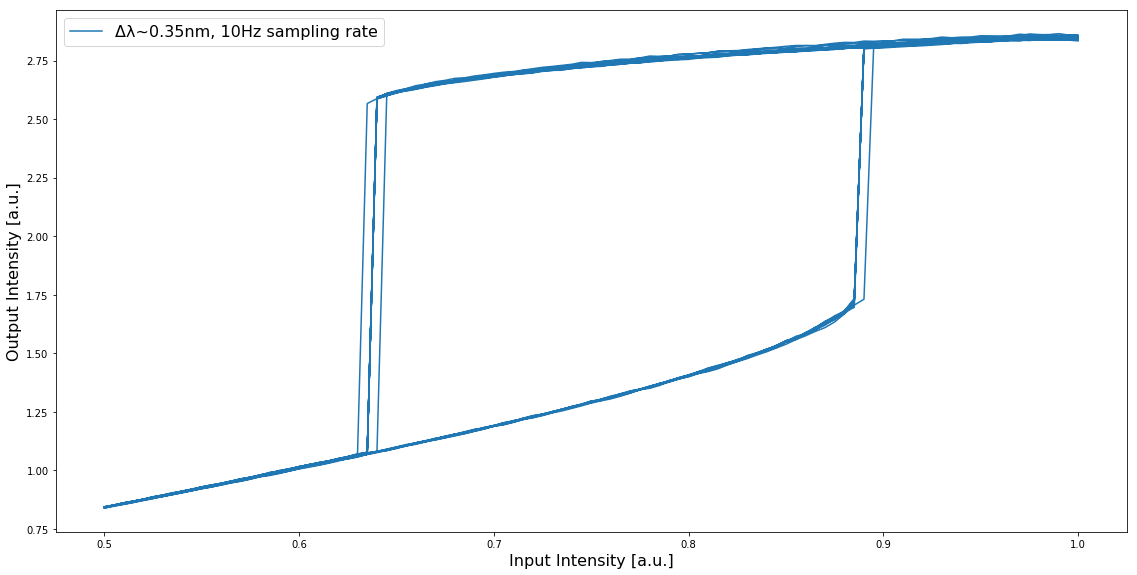
\includegraphics[draft,width=9cm,height=6cm]{figures/foo.png}
	\caption{image/scheme of the slab VG and critical angle.}
	\label{fig:slabVG}
\end{figure}

2D-waveguides on the other hand are more used, since they allow to confine light in a straight path and conduct it to the designed spot.
A few types are shown in \autoref{fig:2DVG} below.

\begin{figure}[ht]
	\centering
	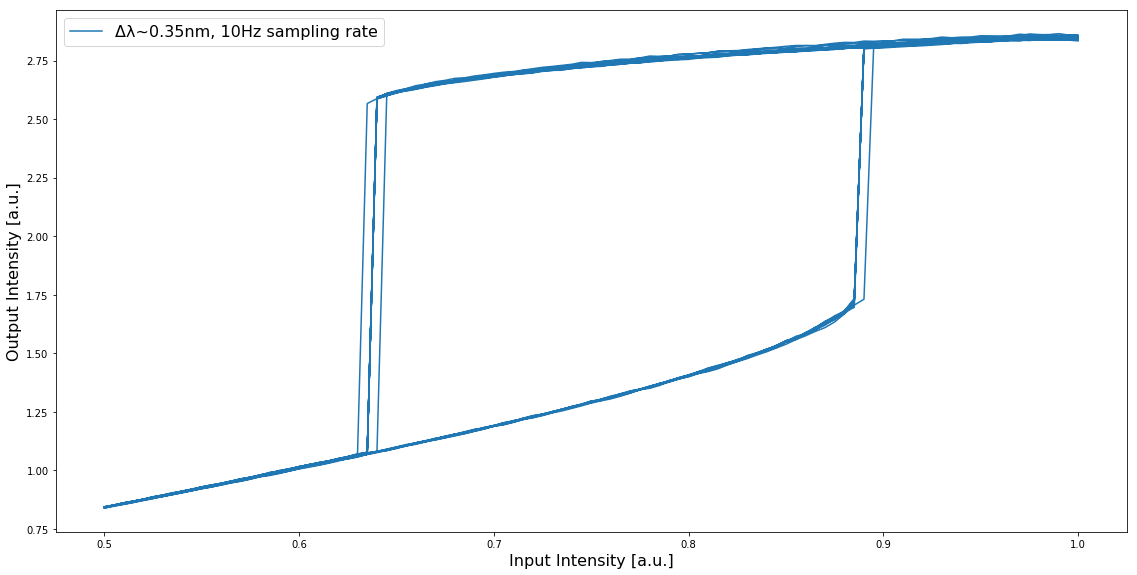
\includegraphics[draft,width=9cm,height=6cm]{figures/foo.png}
	\caption{2D VGs.}
	\label{fig:2DVG}
\end{figure}

\section{Microring Optical Cavity}
\label{sec:Microring_Optical_Cavity}
In integrated photonics the microring is an optical cavity made by bending a waveguide on itself.

\subsection{Nonlinear Perturbations}
\label{ssec:Nonlinear_Perturbations}


\section{Photonics applied to ANNs}
\label{sec:Photonics_applied_to_ANNs}

\subsection{Weighted sum of inputs}
\label{ssec:Weighted_Sum_of_inputs}
This has already been demonstrated and integrated widely, so it will not be the focus of this work.

\subsection{Nonlinear Activation Function}
\label{ssec:Nonlinear_Activation_Function}
As opposed to the mechanism for weighted sum, an phenomenon for the activation function in an integrated photonic circuit has yet to be proposed.

\subsection{Simulations}